
\section{\texttt{lib}}
\lstinputlisting[label={alg:CPU_lib},caption={Implementation of the library function \texttt{cblas\_dgemm}},style=CStyle, linerange={303-313}]{code_3/func_cu.tex}


\newpage
\section{\texttt{jac\_cpu()}}
\lstinputlisting[label={alg:app_jac_v0},caption={Algo. \texttt{jac\_cpu()}.},style=CStyle]{code_3/jac_cpu.c}


\newpage
\section{\texttt{jac\_gpu1()}}
\lstinputlisting[label={alg:app_jac_v1},caption={Algo. \texttt{jac\_gpu1()}.},style=CStyle]{code_3/jac_gpu1.cu}

\newpage
\section{\texttt{jac\_gpu2()}}
\lstinputlisting[label={alg:app_jac_v2},caption={Algo. \texttt{jac\_gpu2()}.},style=CStyle]{code_3/jac_gpu2.cu}


\newpage
\section{\texttt{jac\_gpu3()}}
\lstinputlisting[label={alg:app_jac_v3},caption={Algo. \texttt{jac\_gpu3()}.},style=CStyle]{code_3/jac_gpu3.cu}




\newpage
\section{Visual Estimates of $u(x,y)$}

The following plots in figure \ref{fig:apped_vis_pos} visualizes the estimates of $u(x,y)$ for the four given approaches, \texttt{jac\_cpu}, \texttt{jac\_gpu1}, \texttt{jac\_gpu2} and \texttt{jac\_gpu3}.
The algorithms have been running for $1000$ iterations and for $N=2048$.

\begin{figure}[!th]
\centering
\begin{subfigure}{.5\textwidth}
  \centering
  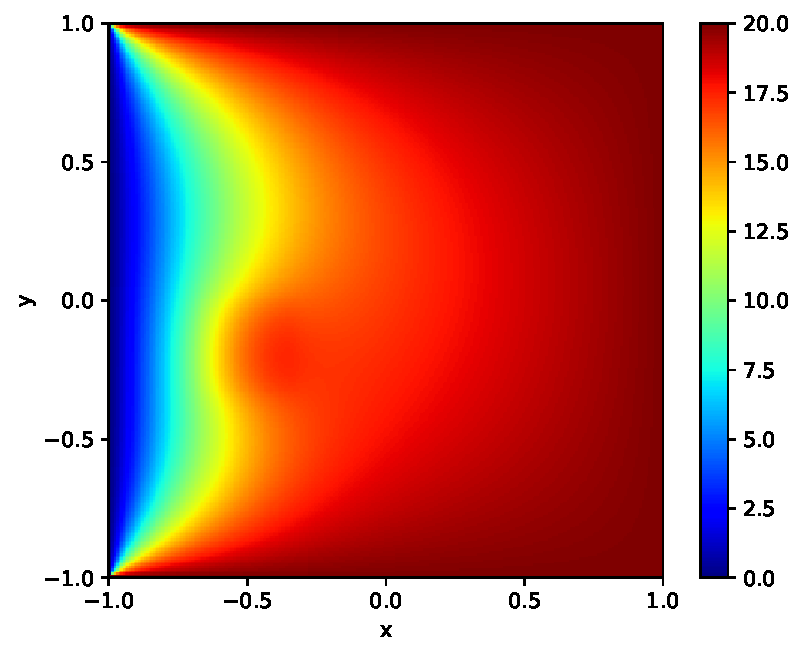
\includegraphics[width=.9\linewidth]{data_3/pos/jac_cpu.pdf}
  \caption{\texttt{jac\_cpu}}
  \label{fig:jac_gpu}
\end{subfigure}%
\begin{subfigure}{.5\textwidth}
  \centering
  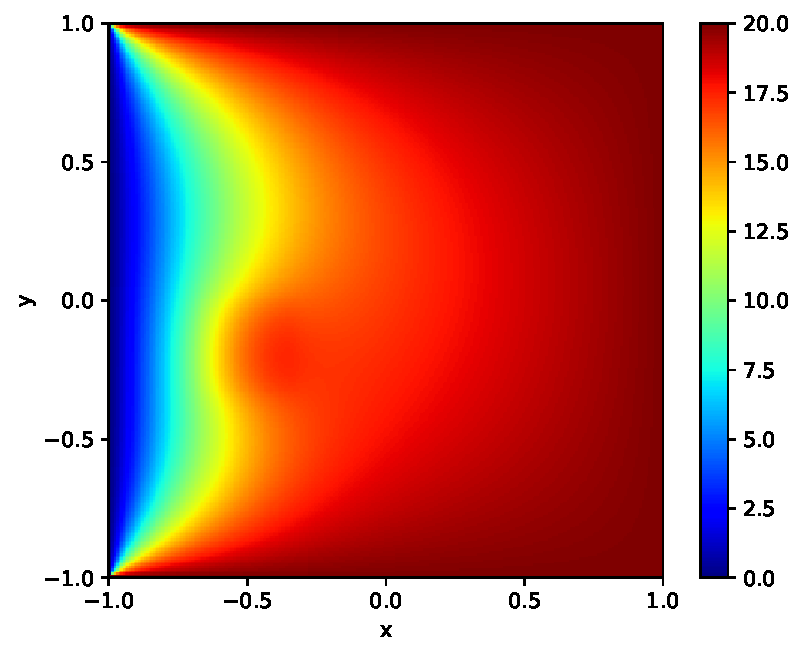
\includegraphics[width=.9\linewidth]{data_3/pos/jac_gpu1.pdf}
  \caption{\texttt{jac\_gpu1}}
  \label{fig:jac_gpu1}
\end{subfigure}
\begin{subfigure}{.5\textwidth}
  \centering
  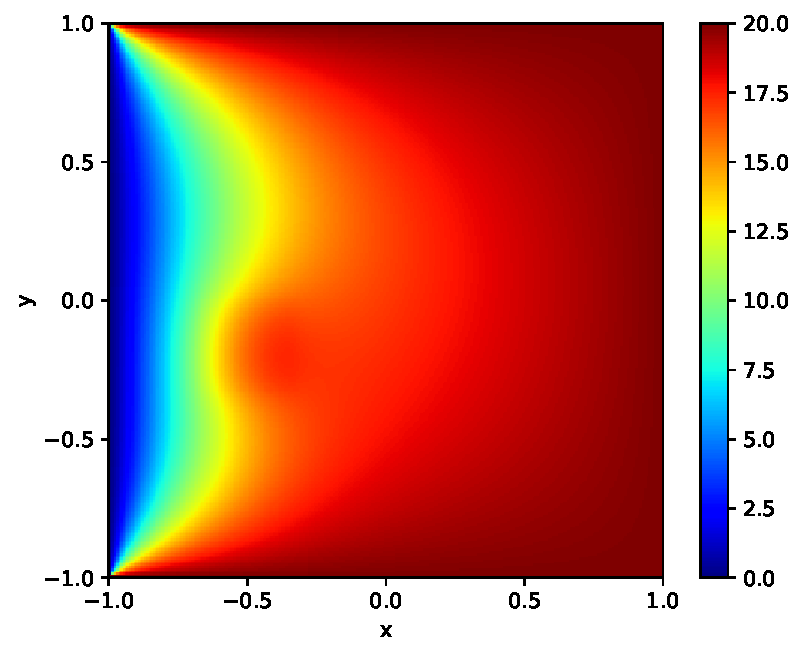
\includegraphics[width=.9\linewidth]{data_3/pos/jac_gpu2.pdf}
  \caption{\texttt{jac\_gpu2}}
  \label{fig:jac_gpu2}
\end{subfigure}%
\begin{subfigure}{.5\textwidth}
  \centering
  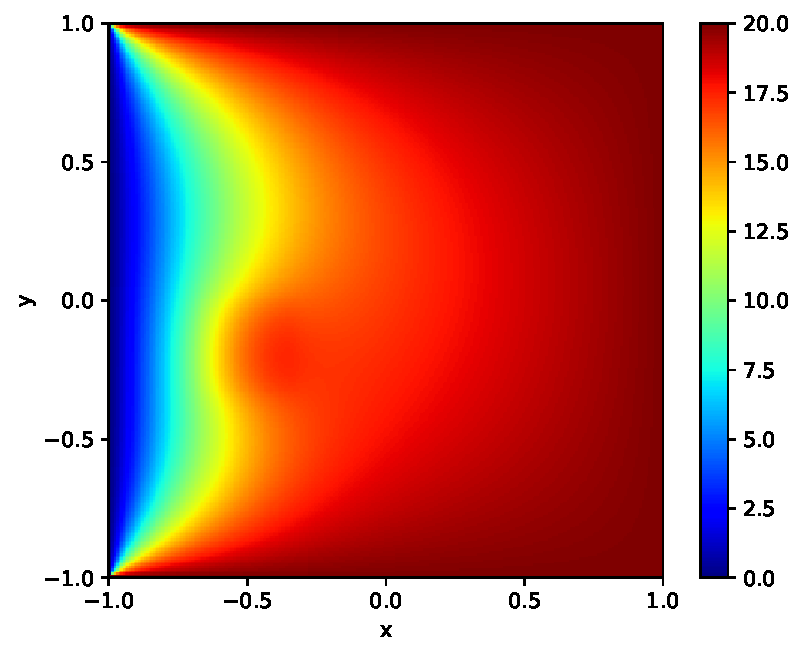
\includegraphics[width=.9\linewidth]{data_3/pos/jac_gpu3.pdf}
  \caption{\texttt{jac\_gpu3}}
  \label{fig:jac_gpu3}
\end{subfigure}
\caption{Estimate of the function $u(x,y)$.}
\label{fig:apped_vis_pos}
\end{figure}